\section{Reto}
\begin{frame}{Reto}
    \Huge\centering\textbf{CHALLENGE TIME!}
\end{frame}

\subsection{Puzles en Profesor Layton}
\begin{frame}{Objetivo}

    {\Large\bfseries Crear un puzle}
    \begin{columns}
    \begin{column}{0.5\textwidth}
        \begin{itemize}
            \item<1-> Título (\textit{script/puzzletitle})
            \item<2-> Localización (\textit{script/qinfo})
            \item<3-> Descripción (\textit{qtext})
            \item<4-> Pistas (\textit{qtext})
            \item<5-> Respuesta (\textit{qtext})
            \item<6-> \textit{Picarats} (\textit{script/pcarot})
            \item<7-> Entrada (\textit{script/qscript})
        \end{itemize}
    \end{column}
    \begin{column}{0.5\textwidth}
        \only<1,2>{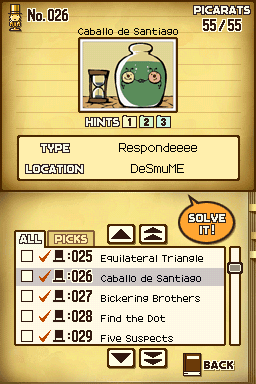
\includegraphics[width=0.7\textwidth]{imgs/reto1.png}}
        \only<3,6>{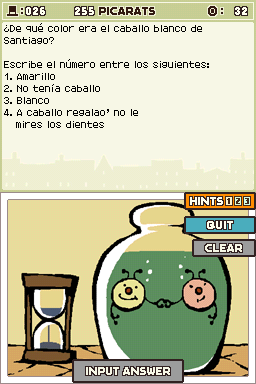
\includegraphics[width=0.7\textwidth]{imgs/reto2.png}}
        \only<4>{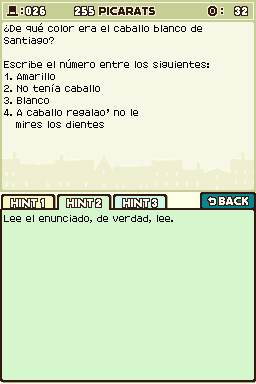
\includegraphics[width=0.7\textwidth]{imgs/reto3.png}}
        \only<7>{\includegraphics[width=0.7\textwidth]{imgs/reto4.png}}
        \only<5>{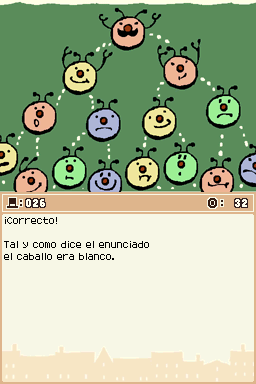
\includegraphics[width=0.7\textwidth]{imgs/reto5.png}}
    \end{column}
    \end{columns}
\end{frame}

\begin{frame}{Pistas sobre los scripts}
    \begin{itemize}
        \visible<+->{\item Primeros 4 bytes es el tamaño del archivo}
        \visible<+->{\item Se compone de múltiples comandos + argumentos}
        \visible<+->{\item Despues de \texttt{0x0000} va el ID del comando}
        \visible<+->{\item El formato de los argumentos es tipo + valor}
        \visible<+->{\item El tipo \texttt{0x0001} es un entero de 32 bits}
        \visible<+->{\item El tipo \texttt{0x0003} es una cadena de caracteres de longitud variable}
        \visible<+->{\item Los scripts terminan con \texttt{0x000C}}
    \end{itemize}
\end{frame}
